%Set document class
\documentclass{article}

%Load math symbol packages
\usepackage{amsmath}
\usepackage{amssymb}
\usepackage{mathtools}
\usepackage{indentfirst}
\usepackage{graphicx}
\usepackage{listings}

%User defined commands
\newcommand{\var}{\operatorname{Var}}
\newcommand{\cov}{\operatorname{Cov}}
\newcommand{\sumN}{\sum_{i=1}^{n}}
\newcommand{\sumM}{\sum_{i=1}^{m}}
\newcommand{\prodN}{\prod_{i=1}^{n}}
\newcommand{\prodM}{\prod_{i=1}^{m}}

\begin{document}
\begin{center}
	\huge{\bf Math 181B: Homework 3} \\
	Merrick Qiu 
\end{center}

\subsection*{Exercise 1}
\begin{align*}
	&P(X_1=a, X_2=b)  \\
	= &\sum_{\substack{(k_3,\hdots,k_t) \\ \sum_{i-3}^t k_i = n-a-b}}
		P((x_1, x_2, x_3, \hdots, x_t) = (a,b,k_3,\hdots,k_t)) \\
	= &\sum_{\substack{(k_3,\hdots,k_t) \\ \sum_{i-3}^t k_i = n-a-b}}
		\frac{n!}{a!b!k_3!\hdots k_t!} p_1^a p_2^b p_3^{k_3} \hdots p_t^{k_t} \\
	= &\frac{n!}{a!b!(n-a-b)!} p_1^a p_2^b (1-p_1-p_2)^{n-a-b} \sum_{\substack{(k_3,\hdots,k_t) \\ \sum_{i-3}^t k_i = n-a-b}}
		\frac{(n-a-b)!}{k_3!\hdots k_t!}  \frac{p_3^{k_3} \hdots p_t^{k_t}}{(1-p_1-p_2)^{n-a-b}} \\
	= &\frac{n!}{a!b!(n-a-b)!} p_1^a p_2^b (1-p_1-p_2)^{n-a-b}
\end{align*}
We have shown that $P(X_1=a, X_2=b)$ has the same 
probability density function as $Multinom(n,p_1,p_2,1-p_1-p_2)$, 
so we have that  $(X_1,X_2,Y) \sim Multinom(n,p_1,p_2,1-p_1-p_2)$.
The last step follows from the fact that the summation is the sum of the probabilities of all
possible outcomes of $Multinom(n-a-b,\frac{p_3}{1-p_1-p_2},\hdots,\frac{p_t}{1-p_1-p_2})$,
which is equal to 1.
\newpage 

\subsection*{Exercise 2}
We have the hypotheses that $H_0: X \sim Poisson(\hat{\lambda})$
and $H_1: $ The model does not fit the data well.
The following code gives a p-value of $0.1231678$,
meaing that we fail to reject the null hypothesis and 
a Poisson fits the distribution.
For the test to work, we assume that $E_i \geq 5$, 
for the distribution to closely match a chi-squared.
This is true for all bins except $E_0 = 4$,
but this should not be a problem since 4 is close to 5.s
\begin{lstlisting}
# Import files
setwd("C:/Users/merri/Documents/MATH-31H/MATH 181B/Homework 3")
x = unlist(read.csv("Question.csv"))

#Estimate MLE for Poisson
lambda_hat = mean(x)

# Put data into bins
bins = c(0,1,2,3,4,5,6,7,Inf)
observed = table(cut(x, bins, right=F))

# Expected probabilities
probabilities = dpois(c(0,1,2,3,4,5,6,Inf), lambda_hat)
probabilities[8] = 1 - ppois(6, lambda_hat)
expected = probabilities*length(x)

#Calculate D
D = sum((observed-expected)^2/expected)

#8-1-1 degrees of freedom
pchisq(D, df=6, lower.tail=FALSE)

#P-value is 0.1231678>0.03
\end{lstlisting}
\newpage 

\subsection*{Exercise 3}
\begin{enumerate}
	\item \begin{lstlisting}
#get a random value for d
getd = function() {
  probs = c(0.3,0.5,0.2)
  observed = rmultinom(1, 50, probs)
  expected = 50*probs
  
  D = sum((observed-expected)^2/expected)
}

# create vector of 1000 samples of D
dvalues = rep(0, 1000)
for (i in 1:1000) {
  dvalues[i] = getd()
}

# Plot histogram
hist(dvalues, breaks = 20, freq=FALSE, main="D histogram")
curve(dchisq(x, df = 2), add = TRUE, col = "red", lwd = 2)
	\end{lstlisting}
	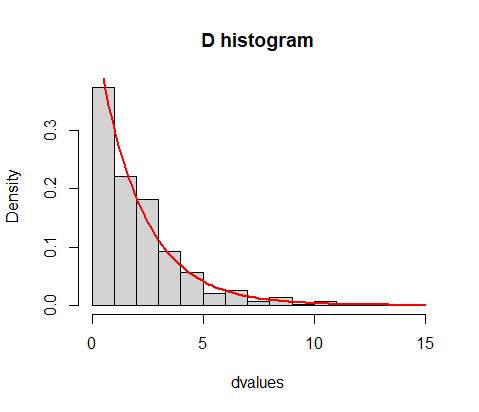
\includegraphics[scale=0.7]{parta.png}

	The histogram matches closely with the chi-squared distribution,
	so my simulation does agree with theory.
	\newpage 
	\item \begin{lstlisting}
# create vector of rejections
rejections = rep(0, 1000)
for (i in 1:1000) {
  dvalue = getd()
  pvalue = pchisq(dvalue, df=2, lower.tail=FALSE)
  if (pvalue < 0.05) {
    rejections[i] = 1
  }
}

sum(rejections)/1000
#0.057
	\end{lstlisting}
	We see that the propotion of rejections is $0.057$,
	which is close to the value of $\alpha$.
	\newpage
	\item 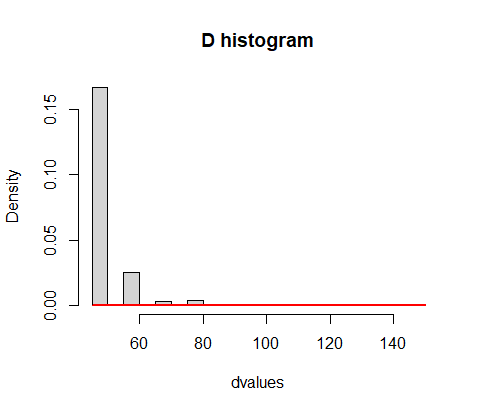
\includegraphics[scale=0.7]{partc.png}
	\item 
	Changing part a) to this distribution yields dvalues that are much much 
	larger than before, in a region where the chi-squared distribution has 
	very low density.

	Changing part b) to this distribution yields a rejection rate of $1$,
	which makes sense considering how large the values of d were.
\end{enumerate}
\end{document}




